\documentclass[conference]{IEEEtran}
\IEEEoverridecommandlockouts
\usepackage{cite}
\usepackage[T1]{fontenc}
\usepackage{lmodern}
\usepackage{amsmath,amssymb}
\usepackage{graphicx}
\usepackage{booktabs}
\usepackage{url}
\usepackage[hidelinks]{hyperref}

\begin{document}

\title{A Local-First Autonomous Trading Research Desk:\\
Sub-Second Voice Control, and What 7{,}312 Forward Tests Showed}

\author{\IEEEauthorblockN{Sai Yaganti}
\IEEEauthorblockA{\textit{Independent Researcher} \\
Vancouver, British Columbia, Canada \\
devicelifecycle@gmail.com}}

\maketitle

\begin{abstract}
We describe AXIOM, a research desk that runs entirely on one workstation: it
places paper trades across seven strategies, keeps a written record of what it
learns, and is operated by speaking to it. Two results are reported. First, a
voice loop built from open models (Whisper through whisper.cpp for listening
and Piper for speaking) answers a spoken question in 0.69 to 1.39 seconds end
to end, with transcription at 105 to 215\,ms, and needs no network and no
third-party service. Reaching that latency required discarding two designs
that appear correct and are not: recording microphone audio with
\texttt{MediaRecorder}, which produces undecodable fragments when an utterance
is cut from the middle of a stream, and gating speech against absolute energy
thresholds, which on the measured hardware could never open. Second, and more
importantly for anyone building such a system, the desk's own record argues
against most of its strategies. Over 61 days and 7{,}312 paper trades the
aggregate profit factor is 0.81 and expectancy is $-\$1.80$ per trade; a Monte
Carlo permutation test clears exactly one of seven strategies as robust and
marks one marginal. The single consistently profitable book is a weather
prediction-market strategy whose edge appears only after an entry gate is
applied: the same signal, ungated, lost $\$212.67$ over 248 trades, and gated,
returned $+\$88.84$ over 279 trades at an 83.5\% hit rate. We argue that the
value of a system like this lies less in the strategies it runs than in the
discipline of forward-testing them honestly in public view, and we report the
negative results in full.
\end{abstract}

\begin{IEEEkeywords}
algorithmic trading, forward testing, speech recognition, voice user
interfaces, on-device inference, prediction markets, Monte Carlo permutation
testing
\end{IEEEkeywords}

\section{Introduction}

A retail algorithmic trader today has no shortage of tools and a serious
shortage of trustworthy evidence. Backtests are cheap, easy to overfit, and
almost always flattering; the literature on this is long and consistent
\cite{bailey2014,harvey2016,white2000}. The honest remedy is forward testing:
run the strategy on data it has never seen, in something close to real
conditions, and keep the record whether or not it is comfortable reading.

This paper describes a system built around that remedy. AXIOM is a single-user
research desk that runs on one Apple Silicon workstation. It hosts seven
strategy daemons that trade on paper against live market data, a reflection
loop that revises their parameters and writes down what it concludes, a live
globe that carries open-source intelligence feeds, and a voice interface
through which the operator asks questions and gives instructions in ordinary
speech.

We make three contributions.

\textbf{A measured local voice loop.} Section~\ref{sec:voice} reports a
complete speech interface covering wake word, barge-in, transcription, language
model and synthesis, running on the operator's own machine with no audio leaving
it. We give the latency budget stage by stage and the accuracy-versus-latency
tradeoff across four speech recognition models.

\textbf{Two negative engineering results that cost real time.} Both concern
designs that look correct in a code review and fail in use. Browser
\texttt{MediaRecorder} output cannot be sliced by a voice activity detector,
because every chunk after the first lacks a container header and, once a header
is restored, carries a timestamp that makes the decoder emit the entire session
as silence. Separately, an energy gate with any absolute threshold is untenable
across microphones: the device measured here peaks at 0.0016\,RMS, so a
threshold of 0.004, a value that seems conservatively low, can never open.

\textbf{A full and unflattering forward-test record.} Section~\ref{sec:results}
reports every strategy the desk runs, including the six that do not survive
their robustness test and the one that lost $\$11{,}277$ before it was retired.

\section{Related Work}

\subsection{Evaluating trading strategies}
The difficulty of distinguishing skill from selection in backtested strategies
is well documented. White's reality check \cite{white2000} and the deflated
Sharpe ratio of Bailey and L\'{o}pez de Prado \cite{bailey2014} both address
the multiple-testing problem directly; Harvey and Liu \cite{harvey2016} argue
that most published factors do not survive an appropriate haircut. Our
robustness gate is a simpler device, a permutation test on trade order from
which we take a probability that the observed win rate arose by chance, but
the motivation is theirs.

\subsection{Open speech models}
Whisper \cite{radford2022} established that a single supervised model can
transcribe robustly across accents and noise; \texttt{whisper.cpp}
\cite{whispercpp} made it practical on consumer CPUs through quantisation and
platform-specific kernels. Piper \cite{piper} provides neural speech synthesis
at similar cost. Both are permissively licensed, which is what makes an
entirely local voice loop possible. Commercial dictation products such as
Wispr Flow are closed, but the open alternatives are built on precisely these
two components.

\subsection{Open-source intelligence feeds}
The globe described in Section~\ref{sec:arch} aggregates public transponder,
orbital and seismic data from OpenSky \cite{opensky}, CelesTrak
\cite{celestrak} and the USGS earthquake feed respectively, in the tradition
of open-source intelligence dashboards. We claim no novelty here; it is context
for the strategies that consume weather and event data.

\section{System Architecture}
\label{sec:arch}

The desk is four layers on one machine.

\textbf{Strategy daemons.} Seven independent processes, each supervised by
\texttt{launchd}, poll their own data sources and write every decision to an
append-only JSON-lines log. A daemon never holds state only in memory; the log
is the record, and every figure in this paper is derived from those logs rather
than from any in-process accounting. We verified this property directly: the
weather book's reported $+\$88.84$ was recomputed from
\texttt{dryrun\_weather.jsonl} by joining each placed bet to the market's own
published resolution and applying the same fee model, and it reproduced to the
cent over the same 279 trades.

\textbf{Reflection loop.} A nightly process reads the logs, fits simple
summaries per strategy and per market segment, and writes back a parameter file
and a dated note in prose. Its conclusions are visible on the desk's home
screen. It concluded, for example, that one city was disabled in the weather book and that
the minimum edge to act was raised to 0.08.

\textbf{Interface.} A Next.js application serves roughly forty pages. Relevant
here are the journal, which renders the forward-test record, and the globe,
which carries the intelligence feeds.

\textbf{Voice.} A bridge process holds the conversation, calls tools on the
operator's behalf, and streams its answer back sentence by sentence. Speech
recognition and synthesis run in a separate always-warm Python service.

\section{The Voice Interface}
\label{sec:voice}

\subsection{Capture}
Audio is taken from the microphone through an \texttt{AudioWorklet}, so that
capture runs on the audio thread and is unaffected by whatever the interface is
rendering. We initially used a \texttt{ScriptProcessorNode} on the main thread;
with the globe and charts animating it dropped buffers, and sentences arrived
at the recogniser chopped into single words.

Frames are held in a ring buffer of 500\,ms so that the first word survives the
delay before the gate opens, and speech is considered finished after 420\,ms of
quiet. The utterance is decimated to 16\,kHz, normalised, and written as a WAV
file in the browser.

\subsection{Why not MediaRecorder}
The obvious implementation records with \texttt{MediaRecorder} at a fixed
timeslice and concatenates the chunks belonging to an utterance. It does not
work, for two reasons that only appear at runtime. The first chunk carries the
WebM header and every later chunk is a bare cluster, so an utterance taken from
the middle of the stream has no header and \texttt{ffmpeg} refuses it outright;
in our case every spoken command failed with HTTP 503. Prepending the stored
header fixes the container but not the content: the cluster retains its
original timestamp, so the decoder emits everything since the session began as
silence, and the recogniser hallucinates over the gap. We observed
\texttt{[MUSIC PLAYING]} and ``I'm on camera'' returned for a four-word
command. Writing PCM directly avoids both problems and costs about twenty lines
of code.

\subsection{Voice activity detection}
The gate is a two-threshold energy detector with hysteresis, and, in the part we got wrong
twice, it is expressed purely as a multiple of the room's
own noise floor, which is tracked continuously, including while the operator is
speaking. Our first version tracked the floor only between utterances. Because
a real microphone never reaches digital silence, the gate then never closed,
and every utterance ran to the fifteen-second ceiling: we measured 467\,KB of
audio sent for a four-word command.

The second version added an absolute term, $\text{floor} \times 3.5 + 0.004$.
On the hardware measured here the microphone peaks at 0.0016\,RMS, so that gate
could not open at all. An absolute energy threshold is not portable across
microphones, gain settings, or how far the speaker sits from the device; we
recommend against one.

\subsection{Barge-in and echo}
The microphone stays open while the system speaks, so the operator can
interrupt mid-sentence, as one would with a person. This means the microphone
also hears the loudspeaker. Browser echo cancellation and a raised gate remove
most of it; the remainder is removed in software.

Our first echo filter compared the transcript against a bag of words the system
had recently spoken and discarded anything overlapping by more than half. This
is wrong in a way that is easy to miss and severe in use: the system talks
about the same subjects the operator asks about. Tested against realistic
follow-ups, it suppressed four of five, including ``pause the flow bot''. The
system ignored its operator precisely when he used its own vocabulary.

Echo is better characterised as the same words in the same \emph{order}, as one
unbroken run. Let $h$ be the transcript and $m$ a recent utterance, both as
word sequences, and let $r(h,m)$ be the length of the longest run of
consecutive positions matching under a fuzzy word comparison. We reject the
transcript when
\begin{equation}
r(h,m) \geq 4 \quad\text{and}\quad \frac{r(h,m)}{|h|} \geq 0.85 .
\end{equation}
Measured against real answers, echo scores 1.00 on this ratio and genuine
follow-ups score between 0.29 and 0.75, so the threshold separates them
cleanly.

\subsection{Addressing}
A wake word starts a conversation but does not punctuate one: for 90 seconds
after any exchange, speech is taken as directed at the system, subject to a
ten-minute ceiling so that a room full of conversation cannot hold the channel
open indefinitely. The wake pattern is deliberately permissive, because the
recogniser's errors are concentrated there. We observed ``Hay Axiom'',
``Axem'', ``Acts him'' and ``action'' for the same name. It also accepts
ordinary forms of address such as ``hey buddy''.

\subsection{Latency}
Fig.~\ref{fig:latency} gives the budget. The dominant fixed cost is the
hold-off that decides speech has ended, which is a design choice rather than a
computation. Transcription of a typical utterance takes 105 to 215\,ms and
synthesis 148 to 360\,ms.

Three implementation details account for most of the improvement over our first
working version. The browser sends 16\,kHz mono PCM, which is what the
recogniser wants, so the service passes samples straight to the model rather
than spawning \texttt{ffmpeg} to convert the audio into the format it was
already in; this alone took transcription from 334\,ms to 105\,ms. Both models
are exercised with a real inference at start-up, because loading a model and
building its compute graph are different things and the operator was paying for
the latter on his first word after every restart. And both run off the event
loop under a lock, because each holds the CPU: before this, a sentence being
spoken blocked transcription of the next thing said, turning a 200\,ms render
into eleven seconds.

\begin{figure}[t]
\centering
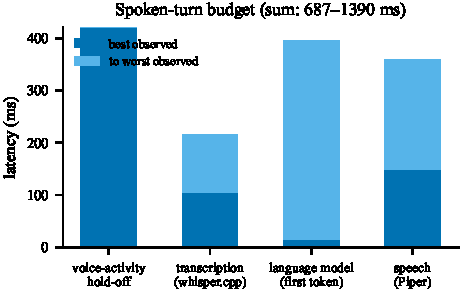
\includegraphics[width=\columnwidth]{fig_latency.pdf}
\caption{Measured latency of each stage of a spoken turn. Bars show the best
and worst observed values over repeated runs on an otherwise loaded
workstation.}
\label{fig:latency}
\end{figure}

\subsection{Choice of recognition model}
Fig.~\ref{fig:asr} plots word error against transcription time for four
Whisper variants on a fixed set of the desk's own commands. The quantised
\texttt{large-v3-turbo} model is perfect on this set and takes 2.17\,s per
utterance; it was CPU-bound and became slower, not faster, with more threads.
The \texttt{base.en} model takes 148\,ms at 5.7\% word error.

That comparison is misleading on its own, because the errors are not uniformly
distributed. Every error \texttt{base.en} made was a spelling of the system's
name. Measured on the remainder of the sentence, the part that determines what
the system actually does, \texttt{base.en} scores 0.0\% word error over the
same set, and correctly recognised that it was being addressed in seven cases
out of seven. We therefore kept the small fast model and widened the wake
pattern, rather than paying 1.3\,s per sentence to have the name spelled
correctly.

\begin{figure}[t]
\centering
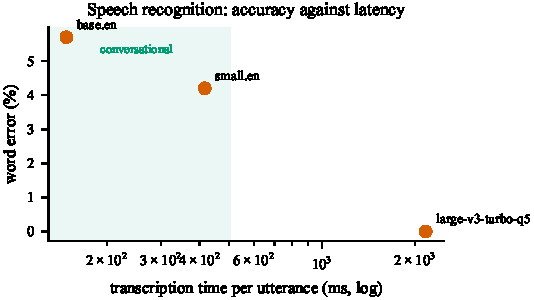
\includegraphics[width=\columnwidth]{fig_asr.pdf}
\caption{Accuracy against latency for four Whisper variants on the desk's own
command set. \texttt{tiny.en} is omitted from the error axis because it failed
to recognise the wake word at all.}
\label{fig:asr}
\end{figure}

\section{Forward-Test Methodology}
\label{sec:method}

Each strategy trades a notional paper account and records every decision.
Position sizes are fixed per strategy (\$10 to \$30) so that results are
comparable and no single book can dominate through leverage. Fills are taken at
the quoted price at decision time; we do not model queue position or partial
fills, which is a real limitation discussed in Section~\ref{sec:limits}.

Fees are charged on every trade. For prediction-market trades we apply the
venue's published formula, which is a function of stake and entry price,
$\text{fee} = 0.018 \times 4 \times s \times p(1-p)$ for stake $s$ at price
$p$. All figures in this paper are after fees. The difference is not cosmetic:
the weather book's gross return of $+\$120.38$ becomes $+\$88.84$ once fees are
applied, a reduction of 26\%.

\textbf{Robustness.} For each strategy we compare the observed win rate against
the distribution obtained by permuting trade outcomes, and report the
probability that the observed result arose by chance. We label a strategy
robust when that probability is small and its expectancy is positive, marginal
when the evidence is weak in either direction, and not robust otherwise. This
is a coarse instrument. It does not correct for the number of strategies
tried, which by the arguments of \cite{harvey2016} it should, and we treat its
verdicts as a filter for attention rather than as proof.

\section{Results}
\label{sec:results}

\subsection{Aggregate}
Table~\ref{tab:overall} gives the desk's whole record. It loses money. Over 61
trading days and 7{,}312 trades the net result is $-\$13{,}133.62$, the profit
factor is 0.81, and the expected value of a trade is $-\$1.80$. The average win
(\$16.78) and average loss (\$17.13) are nearly equal, so with a 45.2\% win
rate the arithmetic is unforgiving.

\begin{table}[t]
\caption{Aggregate forward-test record, 61 days, after fees}
\label{tab:overall}
\centering
\begin{tabular}{lr}
\toprule
Trades & 7{,}312 \\
Win rate & 45.2\% \\
Gross profit & \$55{,}472.47 \\
Gross loss & \$68{,}606.09 \\
Net & $-$\$13{,}133.62 \\
Profit factor & 0.81 \\
Expectancy per trade & $-$\$1.80 \\
Average win / average loss & \$16.78 / \$17.13 \\
Largest win / largest loss & \$1{,}912 / $-$\$2{,}555 \\
Maximum drawdown & \$15{,}418.50 \\
Longest winning / losing run & 21 / 19 \\
\bottomrule
\end{tabular}
\end{table}

\subsection{Where the losses are}
Fig.~\ref{fig:loss} decomposes the gross loss. It is not evenly spread: a
single options strategy accounts for the large majority of it. That strategy
was retired, and the experience is the reason the desk now gates a book on
evidence before letting it run unattended.

\begin{figure}[t]
\centering
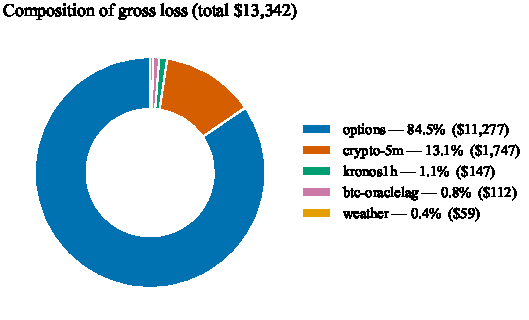
\includegraphics[width=\columnwidth]{fig_loss_pie.pdf}
\caption{Composition of gross loss by strategy. One book dominates; the
remainder are small by comparison.}
\label{fig:loss}
\end{figure}

\subsection{Per strategy}
Fig.~\ref{fig:winrate} shows win rate and robustness verdict for each strategy,
and Table~\ref{tab:strat} the underlying numbers. Of seven strategies, one is
robust, one marginal, and five are not. Two observations are worth drawing out.

A high win rate does not imply a positive expectancy. The weather strategy in
this table wins 63.8\% of its trades and still loses money over the full
period, because it includes the ungated era described below.
Conversely \texttt{vwap-trend} wins under a quarter of its trades and is
mildly profitable, because its winners are large relative to its losers.

The strategy with the most trades is the least robust. \texttt{crypto-5m} has
placed 5{,}658 trades, 77\% of all activity on the desk, at a 45.4\% win rate
for a loss of $\$1{,}747$. Trade count is a measure of activity, not of edge.

\begin{table}[t]
\caption{Per-strategy forward-test record, after fees}
\label{tab:strat}
\centering
\small
\begin{tabular}{lrrrl}
\toprule
Strategy & Trades & Win rate & Net (\$) & Verdict \\
\midrule
crypto-5m      & 5{,}658 & 45.4\% & $-$1{,}747.45 & not robust \\
premarket      &   200 & 40.0\% & $+$112.51 & \textbf{robust} \\
weather        &   527 & 63.8\% & $-$58.86 & not robust \\
kronos1h       &    52 & 38.5\% & $-$146.73 & not robust \\
btc-oraclelag  &   307 & 55.7\% & $-$111.60 & not robust \\
vwap-trend     &   375 & 23.5\% & $+$95.51 & marginal \\
options        &   193 & 22.3\% & $-$11{,}277.00 & not robust \\
\bottomrule
\end{tabular}
\end{table}

\begin{figure}[t]
\centering
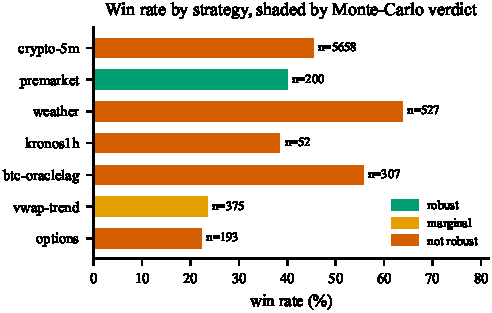
\includegraphics[width=\columnwidth]{fig_winrate.pdf}
\caption{Win rate by strategy with trade counts, shaded by Monte Carlo verdict.
Neither high win rate nor high trade count predicts the verdict.}
\label{fig:winrate}
\end{figure}

\subsection{The one book that works, and why}
The clearest positive result concerns the weather strategy, which bets on
daily maximum-temperature buckets in prediction markets using station
observations and an ensemble forecast. In its first form it traded any bucket
whenever its model disagreed with the market. Over 248 trades it won 41.5\% and
lost $\$212.67$.

The strategy was then gated: it trades only after hour 14 of the local day,
only on favourites priced above 0.75, and only when the modelled edge exceeds
0.18. The rationale is that by mid-afternoon the day's maximum is largely
determined by observations already in hand, so the model's advantage over the
market is real rather than speculative. Under the gate, over 279 trades, it
wins 83.5\% and returns $+\$88.84$ after fees. Fig.~\ref{fig:gate} compares the
two.

The signal did not change. The decision about when to act on it did, and that
is the whole difference between a losing book and a profitable one.

\begin{figure}[t]
\centering
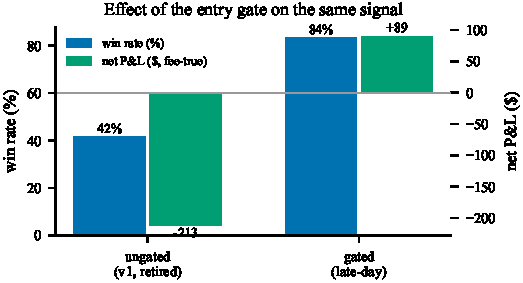
\includegraphics[width=\columnwidth]{fig_gate.pdf}
\caption{The same weather signal before and after an entry gate. Win rate and
fee-true net P\&L over 248 and 279 trades respectively.}
\label{fig:gate}
\end{figure}

\subsection{Diversification}
Fig.~\ref{fig:corr} shows the correlation of daily P\&L between strategies.
Most pairs are near zero and several are negative, which is the property one
wants: the books fail independently. This is cold comfort while the aggregate
expectancy is negative, since uncorrelated losses are still losses, but it means
that if any individual book is fixed, its contribution is additive rather than
redundant.

\begin{figure}[t]
\centering
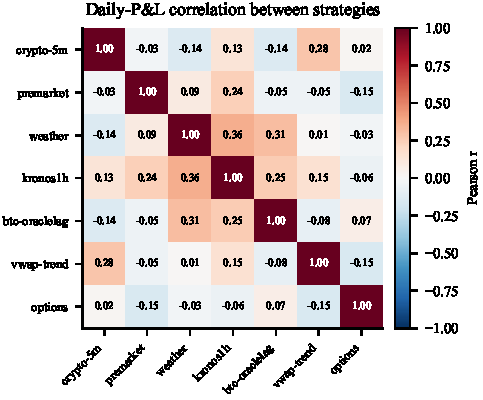
\includegraphics[width=\columnwidth]{fig_corr.pdf}
\caption{Pearson correlation of daily P\&L between strategies. Low correlation
indicates the books are not expressing the same bet.}
\label{fig:corr}
\end{figure}

\subsection{Equity}
Fig.~\ref{fig:equity} shows cumulative paper P\&L. The shape is dominated by
the options book's failure early in the period and flattens once it is retired,
which is the visual signature of a system that stopped a losing strategy rather
than one that found a winning one.

\begin{figure}[t]
\centering
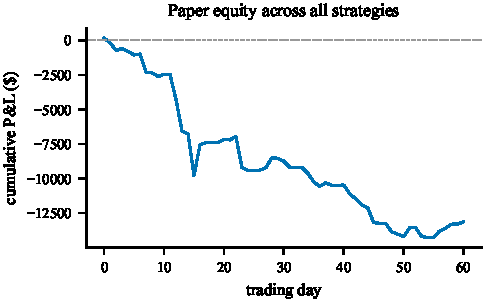
\includegraphics[width=\columnwidth]{fig_equity.pdf}
\caption{Cumulative paper P\&L across all strategies over the 61-day period.}
\label{fig:equity}
\end{figure}

\section{Discussion}

The strategies are mostly bad. We think reporting that plainly is the useful
contribution, because a reader evaluating a similar system will otherwise see
only the one book that works and will draw the wrong conclusion about the base
rate.

What the desk demonstrates is not a source of alpha but a method: run the
strategy forward on unseen data, charge it real fees, write every decision to a
log that can be independently recomputed, and let a robustness test decide
where attention goes. Under that method, six of seven candidate strategies were
identified as not worth capital, one was found to be salvageable by restricting
when it acts, and one modest positive survived. That ratio is consistent with
the multiple-testing literature \cite{harvey2016} and, we suspect, with most
private research that goes unpublished.

The voice interface is a genuine productivity gain, and the reason is latency
rather than novelty. Below roughly a second, asking the desk a question is
cheaper than navigating to the answer, and the operator asks more questions. A
non-trivial amount of the engineering described in Section~\ref{sec:voice}
exists to stay under that threshold without sending audio anywhere.

\section{Limitations and Threats to Validity}
\label{sec:limits}

\textbf{Paper trading is not trading.} We assume fills at the quoted price and
model neither queue position, partial fills, nor market impact. For the weather
strategy, which trades illiquid prediction-market buckets at \$10 a position,
this assumption is optimistic in a way we cannot currently bound.

\textbf{The period is short.} Sixty-one days spans one broad market regime. No
strategy here has been tested across a regime change.

\textbf{The robustness test is coarse.} A permutation test on trade order does
not correct for the number of strategies tried, and by the standards of
\cite{bailey2014} our ``robust'' label is weaker than it sounds. The 200-trade
sample behind that label is small.

\textbf{Single operator, single machine.} All speech measurements come from one
speaker, one microphone and one workstation. The microphone level that broke
our energy gate is one data point; we report it because an absolute threshold
failed, not because 0.0016\,RMS is representative.

\textbf{Venue access is a live constraint.} The only consistently profitable
strategy trades a venue that is not legally accessible from the operator's
jurisdiction, which is an unresolved practical problem and not merely an
administrative one.

\section{Conclusion}

We built a research desk that runs on one machine, speaks and listens without a
network, and keeps an auditable record of every trade it places. The voice loop
answers in about a second, and getting there was mostly a matter of discarding
two plausible designs, container-based audio capture and absolute energy
gating, that fail for reasons invisible until they are measured.

The trading record is negative in aggregate and we report it in full: 7{,}312
trades, a profit factor of 0.81, and one strategy in seven surviving its
robustness test. The one book that does work became profitable not through a
better model but through a restriction on when it is allowed to act. We think
that is the most transferable finding here, and we would rather publish it
alongside the losses than on its own.

\section*{Availability}

The desk, including the strategy daemons, the voice service and the analysis
used for every figure in this paper, is maintained as a single repository. All
figures are generated directly from the live logs by the script accompanying
this paper; no values were transcribed by hand.

\begin{thebibliography}{00}

\bibitem{white2000} H. White, ``A reality check for data snooping,''
\emph{Econometrica}, vol.~68, no.~5, pp.~1097--1126, 2000.

\bibitem{bailey2014} D.~H. Bailey and M. L\'{o}pez de Prado, ``The deflated
Sharpe ratio: correcting for selection bias, backtest overfitting, and
non-normality,'' \emph{Journal of Portfolio Management}, vol.~40, no.~5,
pp.~94--107, 2014.

\bibitem{harvey2016} C.~R. Harvey, Y. Liu, and H. Zhu, ``$\ldots$ and the
cross-section of expected returns,'' \emph{Review of Financial Studies},
vol.~29, no.~1, pp.~5--68, 2016.

\bibitem{radford2022} A. Radford, J.~W. Kim, T. Xu, G. Brockman, C. McLeavey,
and I. Sutskever, ``Robust speech recognition via large-scale weak
supervision,'' arXiv:2212.04356, 2022.

\bibitem{whispercpp} G. Gerganov, ``whisper.cpp: port of OpenAI's Whisper model
in C/C++,'' 2023. [Online]. Available:
\url{https://github.com/ggerganov/whisper.cpp}

\bibitem{piper} M. Hansen, ``Piper: a fast, local neural text-to-speech
system,'' 2023. [Online]. Available:
\url{https://github.com/rhasspy/piper}

\bibitem{opensky} M. Sch\"{a}fer, M. Strohmeier, V. Lenders, I. Martinovic, and
M. Wilhelm, ``Bringing up OpenSky: a large-scale ADS-B sensor network for
research,'' in \emph{Proc. IPSN}, 2014, pp.~83--94.

\bibitem{celestrak} T.~S. Kelso, ``CelesTrak: orbital element sets,'' [Online].
Available: \url{https://celestrak.org}

\end{thebibliography}

\end{document}
